\section{Component Architecture} \label{sc:component_architecture}
\begin{figure}[H]
    \centering
    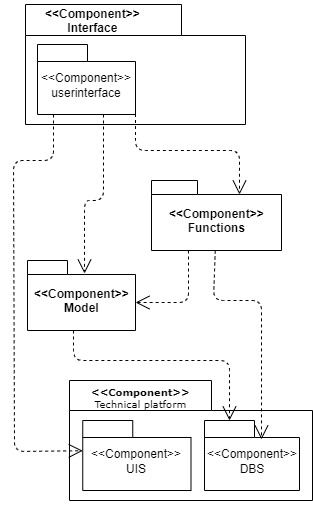
\includegraphics[width=0.6\textwidth]{figures/Componentdiagram.jpg}
    \caption{Component diagram for the Field Component}
    \label{fig:ComponentDesign}
\end{figure}
As seen on \ref{fig:ComponentDesign} the architecture of the system closely resembles the "Generic Architecture Pattern" described in \todo[inline]{Tilføj reference til OOA\&D side 198}.
On the bottom is the database layer, which contains representations of the objects within the program. These representations get converted into accessible and usable objects via the Model layer. The function of the model layer is to convert the representations into objects, which the functions component can utilize and manipulate. Based on the instructions from the interface component, the function layer will manipulate or add objects from the model layer.